% DOC SETTINGS ===================================
\documentclass{article}
\usepackage[utf8]{inputenc}
\usepackage{steinmetz}
\usepackage{mathtools}  
\usepackage{multicol}
\usepackage{circuitikz}
\usepackage{tikz}
\usepackage{listings}
\usepackage{geometry}
\usepackage{fancyhdr}
\usepackage{amsfonts}
\usepackage{media9}
\usepackage{parskip}
\usetikzlibrary{positioning, fit, calc}
\pagestyle{fancy}
\lhead{ECE2714 Problem Set 7}
\rhead{Kavin Thirukonda 2021}
\fancyheadoffset{0mm}
 \geometry{
 a4paper,
 total={170mm,257mm},
 left=20mm,
 top=25mm,
 }
\mathtoolsset{showonlyrefs} 
\cfoot{}
% DOC SETTINGS ===================================
\begin{document}
\begin{enumerate}
    \item Consider a periodic pulse signal x(t) with period T=1 given by 
    \begin{equation}
        x(t) = \sum_{m=-\infty}^\infty x_p(t-m)
    \end{equation}
    where
    \begin{equation}
        x_p(t) = \begin{cases}
        1 & 0 < t < \frac{1}{2}\\
        0 & -\frac{1}{2} < t < 0
        \end{cases}
    \end{equation}
    Write the Fourier series corresponding to x(t) as a sum of weighted exponential functions.
    \begin{equation}
        a_0 = \int_{-\frac{1}{2}}^{\frac{1}{2}} x(t)dt = \frac{1}{2}
    \end{equation}
    \begin{center}
        if T = 1, $\omega_o = 2\pi$
    \end{center}
    \begin{align}
        a_k &= \frac{1}{T}\int_{T} x(t)e^{-jk\omega_ot}dt\\ 
        &= \frac{1}{2T}\int_{T} e^{-jk\omega_ot}dt\\
        &= \frac{1}{2T}\int_{T} \cos(k\omega_ot) - \underbrace{j\sin(k\omega_ot)}_{=0}dt\\
        &= \frac{1}{2T} \frac{1}{k\omega_o}\sin(k\omega_ot)\bigg|_{-\frac{1}{2}}^{\frac{1}{2}}\\
        &= \frac{1}{2kT\omega_o}(\sin(k\omega_o\frac{1}{2})-\sin(-k\omega_o\frac{1}{2}))\\
        &= \frac{2\sin(\frac{k2\pi}{2})}{2kT\omega_o}\\
        &= \frac{\sin(k\pi)}{k2\pi}
    \end{align}
    \begin{equation}
        x(t) = \boxed{\sum_{k=-\infty}^\infty \frac{\sin(k\pi)}{k2\pi}e^{j2\pi kt}, \text{ for k = 0, } \frac{\sin(k\pi)}{k2\pi} = \frac{1}{2}}
    \end{equation}
    \newpage
    \item Plot the amplitude an phase spectrum of the signal in problem 1 for values of k from -10 to 10.
    \begin{equation}
        \boxed{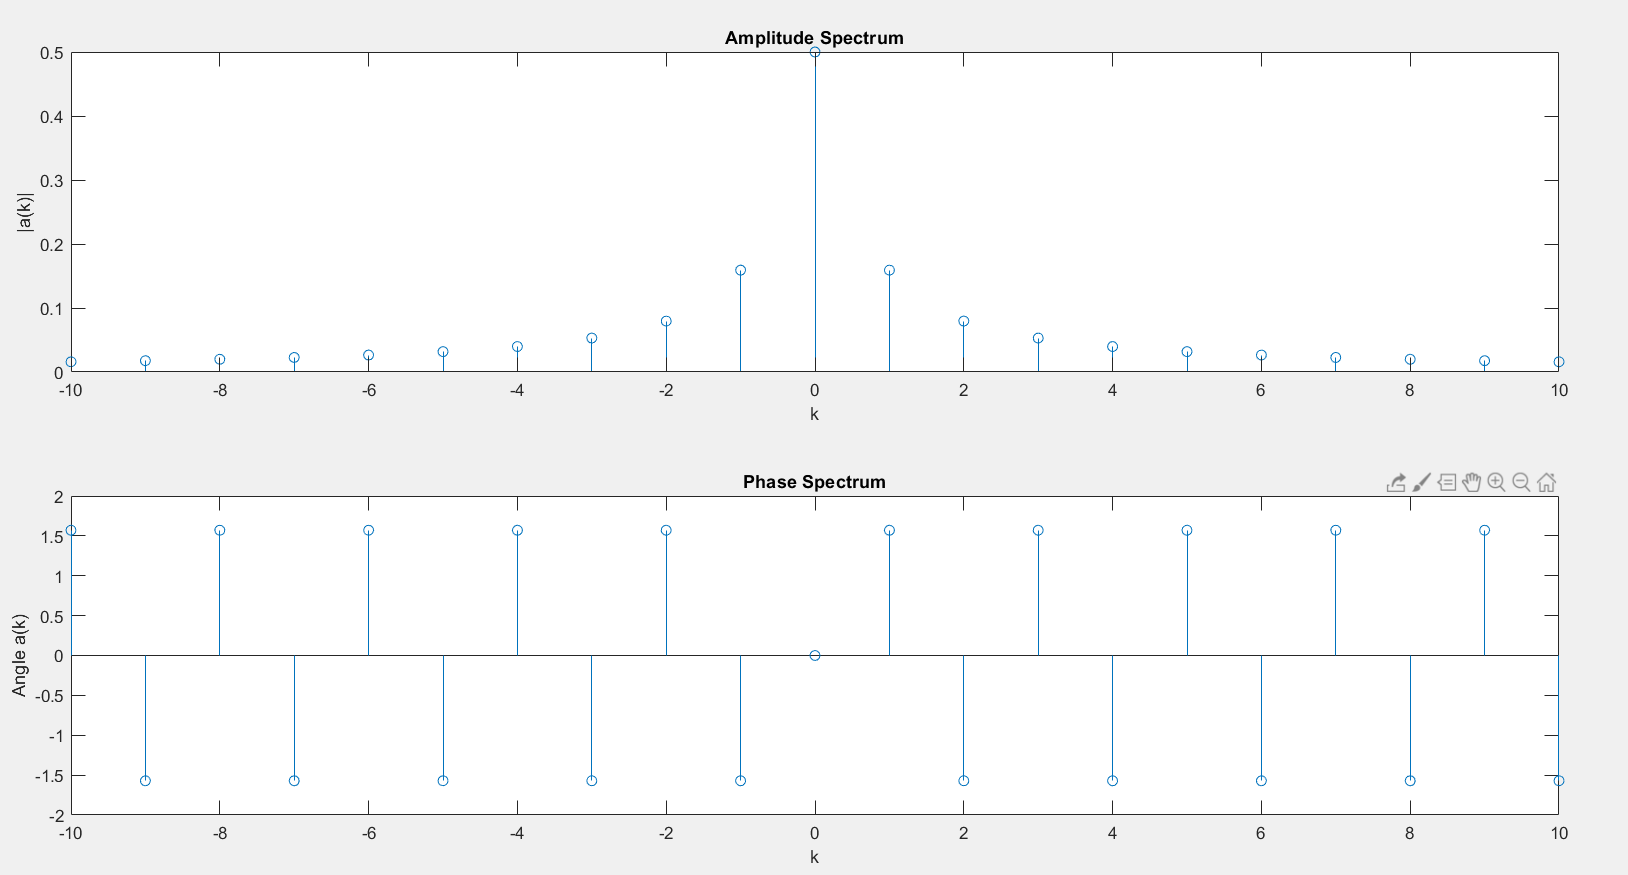
\includegraphics[width = .75\textwidth]{coeff.png}}
    \end{equation}
    \item Plot the Fourier series representation of the result in problem 1 over one period, truncated to $N = \pm 5$ terms, overlayed with the original signal
    \begin{center}
        \boxed{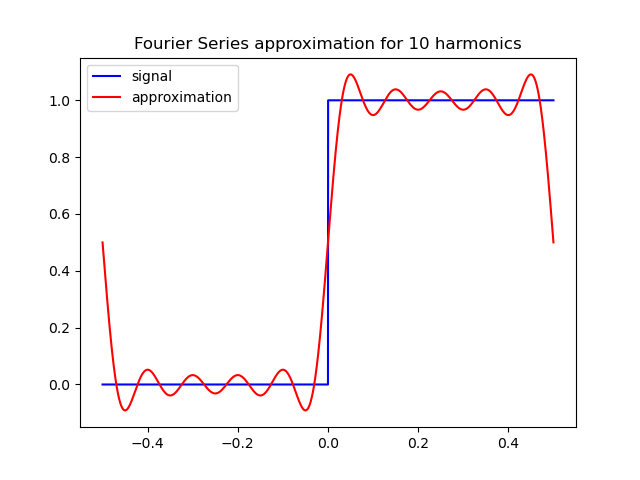
\includegraphics[width = .5\textwidth]{fourier.png}}
    \end{center}
    \newpage
    \item Consider a periodic signal x(t) with fundamental frequency given by $\omega_o= 2\pi$,
    \begin{equation}
        x(t) = \sum_{k=-3}^3 a_ke^{jk2\pi t},
    \end{equation}
    where $a_o = 1, a_1 =\frac{1}{4}, a_{-1}=\frac{1}{4}, a_2 = \frac{1}{4}, a_2 = \frac{1}{5}, a_{-2} = \frac{1}{5}, a_3 = \frac{1}{6}, a_{-3} = \frac{1}{6}$. Write x(t) as a function of sine and cosine functions.
    \begin{align}
        x(t) &= \sum_{k=-3}^3 a_ke^{jk2\pi t}\\
        &= a_{-3}e^{jk2\pi t}+a_{-2}e^{jk2\pi t} + a_{-1}e^{jk2\pi t} + a_{0}e^{jk2\pi t} + a_{1}e^{jk2\pi t} +  a_{2}e^{jk2\pi t} + a_{3}e^{jk2\pi t}\\
        &= \frac{1}{6}e^{jk2\pi t} + \frac{1}{5}e^{jk2\pi t} + \frac{1}{4}e^{jk2\pi t} + e^{jk2\pi t} + \frac{1}{4}e^{jk2\pi t} +  \frac{1}{5}e^{jk2\pi t} + \frac{1}{6}e^{jk2\pi t}\\
        &= \frac{1}{6}(cos(k2\pi t)+jsin(k2\pi t))+ \frac{1}{5}(cos(k2\pi t)+jsin(k2\pi t))\\ &+ \frac{1}{4}(cos(k2\pi t)+jsin(k2\pi t))+ (cos(k2\pi t)+jsin(k2\pi t))+ \frac{1}{4}(cos(k2\pi t)+jsin(k2\pi t))\\ &+  \frac{1}{5}(cos(k2\pi t)+jsin(k2\pi t))+ \frac{1}{6}(cos(k2\pi t)+jsin(k2\pi t))\\
    \end{align}
    \newpage
    \item Consider a periodic signal x[n] with fundamental frequency given by $\omega_o = 2\pi$,
    \begin{equation}
        x[n] = \sum_{k=-2}^2a_ke^{jk2\pi n},
    \end{equation}
    where $a_o = 1, a_1 = \frac{1}{4}, a_{-1} = \frac{1}{4}, a_2 = \frac{1}{5},$ and $a_{-2} = \frac{1}{5}$. Write x[n] as a function of sine and cosine functions.
        \begin{align}
        x[n] &= \sum_{k=-3}^3 a_ke^{jk2\pi t}\\
        &= a_{-2}e^{jk2\pi n} + a_{-1}e^{jk2\pi n} + a_{0}e^{jk2\pi n} + a_{1}e^{jk2\pi n} +  a_{2}e^{jk2\pi n}\\
        &= \frac{1}{5}e^{jk2\pi n} + \frac{1}{4}e^{jk2\pi n} + e^{jk2\pi n} + \frac{1}{4}e^{jk2\pi n} +  \frac{1}{5}e^{jk2\pi n}\\
        &= \frac{1}{5}(\cos(k2\pi n)+j\sin(k2\pi n)) + \frac{1}{4}(\cos(k2\pi n)+j\sin(k2\pi n)) \\ &+ (\cos(k2\pi n)+j\sin(k2\pi n))+ \frac{1}{4}(\cos(k2\pi n)+j\sin(k2\pi n)) \\ &+  \frac{1}{5}(\cos(k2\pi n)+j\sin(k2\pi n))\\
    \end{align}
    \newpage
    \item Consider the periodic DT signal
    \begin{equation}
        x[n] = \sum_{m=-\infty}^\infty z[n-5m]
    \end{equation}
    Where z[n] = $\delta[n+1] - \delta[n]+\delta[n-1].$ Write the DTFS as the solution of a system of linear equations. Using Matlab or similar tool, solve this system of equations to find the Fourier series coefficients.
    \begin{align}
        &x[-2] = \sum_{k=-2}^{2} a_ke^{jk\frac{-4\pi}{5}} = a_{-2}e^{j*-2*\frac{-4\pi}{5}} + a_{-1}e^{j*-1*\frac{-4\pi}{5}} + a_0 + a_1e^{j*1*\frac{-4\pi}{5}} + a_2e^{j*2*\frac{-4\pi}{5}} = 0\\
        &x[-1] = \sum_{k=-2}^{2} a_ke^{jk\frac{-2\pi}{5}} = a_{-2}e^{j*-2*\frac{-2\pi}{5}} + a_{-1}e^{j*-1*\frac{-2\pi}{5}} + a_0 + a_1e^{j*1*\frac{-2\pi}{5}} + a_2e^{j*2*\frac{-2\pi}{5}} = 1\\
        &x[0] = \sum_{k=-2}^{2} a_k = a_{-2} + a_{-1} + a_0 + a_1 + a_2 = -1\\
        &x[1] = \sum_{k=-2}^{2} a_ke^{jk\frac{2\pi}{5}} = a_{-2}e^{j*2*\frac{2\pi}{5}} + a_{-1}e^{j*1*\frac{2\pi}{5}} + a_0 + a_1e^{j*1*\frac{2\pi}{5}} + a_2e^{j*2*\frac{2\pi}{5}} = 1\\
        &x[2] = \sum_{k=-2}^{2} a_ke^{jk\frac{4\pi}{5}} = a_{-2}e^{j*-2*\frac{4\pi}{5}} + a_{-1}e^{j*-1*\frac{4\pi}{5}} + a_0 + a_1e^{j*1*\frac{4\pi}{5}} + a_2e^{j*2*\frac{4\pi}{5}} = 0\\
    \end{align}
    \begin{equation}
        \begin{pmatrix}1&e^{-2\cdot \frac{-4\pi i}{5}}&e^{\frac{4\pi \:i}{5}}&e^{\frac{-4\pi \:i}{5}}&e^{2\cdot \frac{-4\pi \:i}{5}}&0\\ \:\:1&e^{-2\cdot \frac{-2\pi i}{5}}&e^{\frac{2\pi \:i}{5}}&e^{\frac{-2\pi \:i}{5}}&e^{2\cdot \frac{-2\pi \:i}{5}}&1\\ \:\:1&1&1&1&1&-1\\ \:\:1&e^{-2\cdot \frac{2\pi \:i}{5}}&e^{-\frac{2\pi \:i}{5}}&e^{\frac{2\pi \:i}{5}}&e^{2\cdot \frac{2\pi \:i}{5}}&1\\ \:\:1&e^{-2\cdot \frac{4\pi \:i}{5}}&e^{-\frac{4\pi \:i}{5}}&e^{\frac{4\pi \:i}{5}}&e^{2\cdot \frac{4\pi \:i}{5}}&0\end{pmatrix}
    \end{equation}
    \begin{center}
        okay i realized that the summation should go from 0 to 4 instead of -2 to 2 but im not about to rewrite everything i just typed but the answer i got when doing it correctly is below:
    \end{center}
    \begin{align}
        a_{0} = .2\\
        a_{1} = -.0764\\
        a_{2} = -.5236\\
        a_{3} = -.5236\\
        a_{4} = -.0764\\
    \end{align}
\end{enumerate}
\end{document}
